\documentclass[a4paper,12pt]{report}
\usepackage[utf8]{inputenc}
\usepackage[T2A]{fontenc}
\usepackage[russian]{babel}
\usepackage{amsmath}
\usepackage{amssymb}
\usepackage{graphicx}
\usepackage{array}
\usepackage{multirow}
\usepackage{booktabs}
\usepackage{geometry}
\usepackage{float}
\usepackage{ulem}
\usepackage{tabularx}
\usepackage{booktabs}
\usepackage{siunitx}
\usepackage{indentfirst}
\usepackage{placeins}
\usepackage{lipsum}
\usepackage{longtable}
\usepackage{csquotes}
\usepackage[style=gost-numeric,sorting=none]{biblatex}
\usepackage{enumitem}




\addbibresource{references.bib}
\usepackage{titlesec}
\titleformat{\chapter}[display]
    {\normalfont\huge\bfseries}
    {\chaptertitlename\ \thechapter}
    {20pt}
    {\Huge}
\usepackage{booktabs}
\usepackage{makecell}
\graphicspath{{Image/}}

\geometry{
    a4paper,
    total={170mm,257mm},
    left=20mm,
    top=20mm,
}

\newcommand{\specialcell}[2][c]{%
    \begin{tabular}[#1]{@{}c@{}}#2\end{tabular}%
}

\usepackage{etoolbox}
\patchcmd{\thebibliography}
  {\chapter*{\bibname}}
  {\section*{\centering СПИСОК ЛИТЕРАТУРЫ}}
  {}{}
\patchcmd{\thebibliography}
  {\addcontentsline{toc}{chapter}{\bibname}}
  {\addcontentsline{toc}{section}{СПИСОК ЛИТЕРАТУРЫ}}
  {}{}


\usepackage{setspace}
\onehalfspacing


\begin{document}





\begin{center}
    \begin{tabular}{cc}

        \specialcell{
\includegraphics[width=0.8in,height=0.9in]{images/BMSTU.jpg}} & 
        \specialcell{
            \textbf{Министерство науки и высшего образования Российской Федерации} \\
            \textbf{Федеральное государственное автономное образовательное учреждение} \\
            \textbf{высшего образования} \\
            \textbf{«Московский государственный технический университет} \\
            \textbf{имени Н. Э. Баумана} \\
            \textbf{(национальный исследовательский университет)»} \\
            \textbf{(МГТУ им. Н. Э. Баумана)}
        } \\
   
    \end{tabular}
\end{center}

\vspace{1cm}

\begin{center}
    \textbf{ФАКУЛЬТЕТ \uline{«СПЕЦИАЛЬНОЕ МАШИНОСТРОЕНИЕ»}}
    
    \textbf{КАФЕДРА \uline{«РАКЕТНЫЕ И ИМПУЛЬСНЫЕ СИСТЕМЫ» (СМ-6)}}
    
    \vspace{1cm}
    
    \textbf{ДОМАШНЕЕ ЗАДАНИЕ}
    
    \vspace{1cm}
    
    ПО ДИСЦИПЛИНЕ:
    
    \vspace{0.5cm}
    
    \begin{tabular}{c}
       
        \specialcell{Проектирование ракетного оружия} \\
        \hline
    \end{tabular}
    
    \vspace{1cm}
    
    НА ТЕМУ:
    
    \vspace{0.5cm}
    
    \begin{tabular}{c}
       
        \specialcell{Массовый анализ AIM-120 AMRAAM} \\
        \hline
    \end{tabular}
    
    \vspace{1cm}

    
    \vspace{1cm}
    

    \begin{tabular}{llp{3cm}l}
       
        Выполнил: студент группы СМ6-62 & 
        (подпись, дата) & 
         & 
        Ерофеев М.В.\\
        \hline
    \end{tabular}
    
    \vspace{1cm}
    
    \begin{tabular}{llp{3cm}l}
    
        Проверил &  (подпись, дата) & & Лаптева Л.А.\\
        \hline
    \end{tabular}
    
    \vspace{6cm}
    
    Москва, 2025 г.
\end{center}
\tableofcontents

\newpage
\chapter*{Принятые сокращения}
\begin{description}[font=\normalfont\itshape] % обычный шрифт + курсив
\item[WDU] — Weapons Detonation Unit (блок подрыва боевой части)
\item[WGU] — Weapons Guidance Unit (блок наведения вооружения)
\item[WPU] — Weapons Propulsion Unit (двигательный отсек вооружения)
\item[ICPU] — Integrated Control and Power Unit (встроенный блок управления и питания)
\item[РДТТ] — ракетный двигатель твердого топлива
\item[БЧ] — боевая часть
\end{description}


\newpage
\chapter{Краткие сведения о прототипе}
\section{Обзор прототипа}
Ракета AIM-120A AMRAAM (Advanced Medium-Range Air-to-Air Missile –усовершенствованная ракета класса "воздух-воздух"  средней дальности) выполнена по нормальной аэродинамической схеме с «Х» – образным расположением консолей крыла и рулей.

\begin{figure}[h!]
\centering
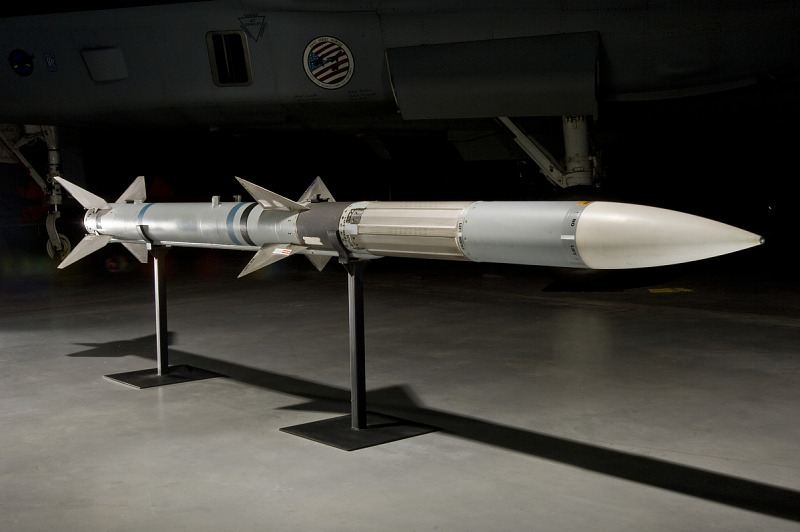
\includegraphics[width=0.7\textheight]{images/1.jpg}
\caption{Ракета AIM-120 AMRAAM}
\label{AIM-120}
\end{figure}

\newpage
\section{Внешнее описание}
Ракета цилиндрическая, длинная, со стреловидным обтекателем.
Носовая часть имеет длину 18.5 дюймов и окрашена в белый цвет. Далее расположена секция батарей серого цвета длиной 17.5 дюймов. Имеется желтая и чёрная полоса с надписью «Осторожно — Используйте защитный чехол для обтекателя».
Следом идет неокрашенная серая секция управления (WCU) длиной 18.75 дюймов. За ней расположена секция БЧ (WDU), длиной 9.5 дюймов, темно-серого цвета.
Эта секция снизу переходит в более светло-серую секцию РДТТ (WPU) длиной 74.75 дюймов. На ней в верхней части расположена черная и синяя полосы, обозначающие, что это учебный снаряд.
За секцией РДТТ находится секция управления рулями длиной 14.75 дюймов. Рули длинные, частично треугольной формы с прямым краем сверху. На них наклеены красно-белые полосы и нанесены номера.
Передние крылья также имеют наклейки и номера. Они алюминиевые, треугольной формы. На ракете присутствуют ушки для крепления к пилону.


\begin{figure}[h!]
\centering
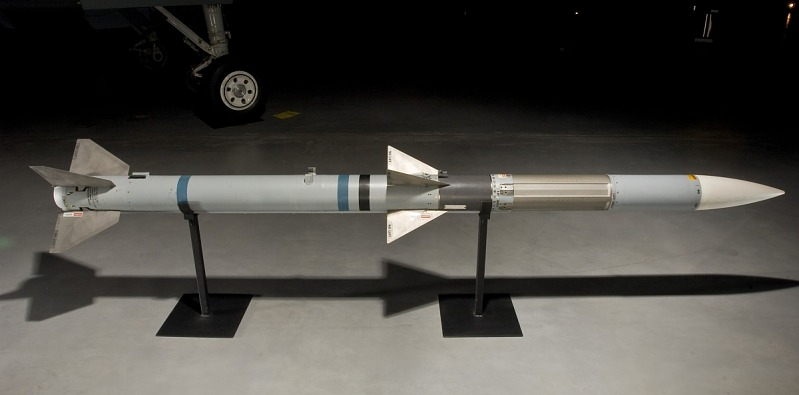
\includegraphics[width=0.55\textheight]{images/2.jpg}
\caption{Ракета AIM-120 AMRAAM}
\label{AIM-120}
\end{figure}

\begin{figure}[h!]
\centering
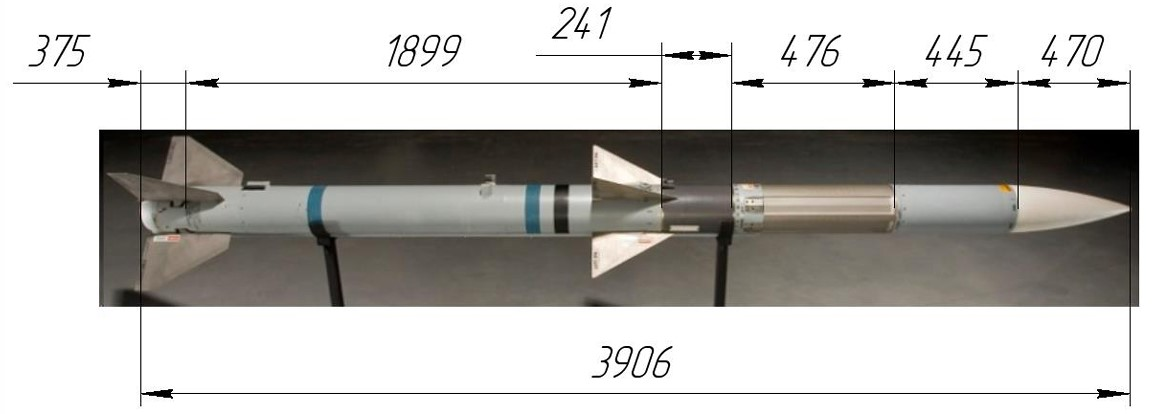
\includegraphics[width=0.65\textheight]{images/3.jpg}
\caption{Размеры отсеков в миллиметрах}
\label{AIM-120}
\end{figure}

\newpage
\section{Внутрення компоновка}
На рисунке 1.4 представлена внутрення компоновка AIM-120, перевод названий модулей дан ниже.

\begin{figure}[h!]
\centering
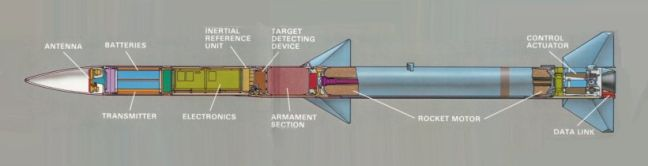
\includegraphics[width=0.7\textheight]{images/4.jpg}
\caption{Компоновка ракеты AIM-120}
\label{AIM-120}
\end{figure}

\begin{description}[font=\normalfont\itshape] % обычный шрифт + курсив
\item[Antenna] — антенна головки самонаведения
\item[(Thermal) batteries] — пиротехнические баратареи, часть ICPU
\item[Transmitter] — передатчик, излучатель
\item[Electronics] — электроника 
\item[Inertial Reference Unit (IRA)] — инерциальная система наведения 
\item[Target Detecting Device (TDD)] — устройство обнаружения цели
\item[Armament Section] — боевая часть 
\item[Rocket Motor] — РДТТ
\item[Contol Actuator] — рулевая машинка
\item[Data Link] — канал передачи данных 
\end{description}

Ниже на рисунке 1.5 представлено разбиение компоновки ракеты на 4 отсека в соответсвии с требованиями ДЗ.

\begin{figure}[H]
\centering
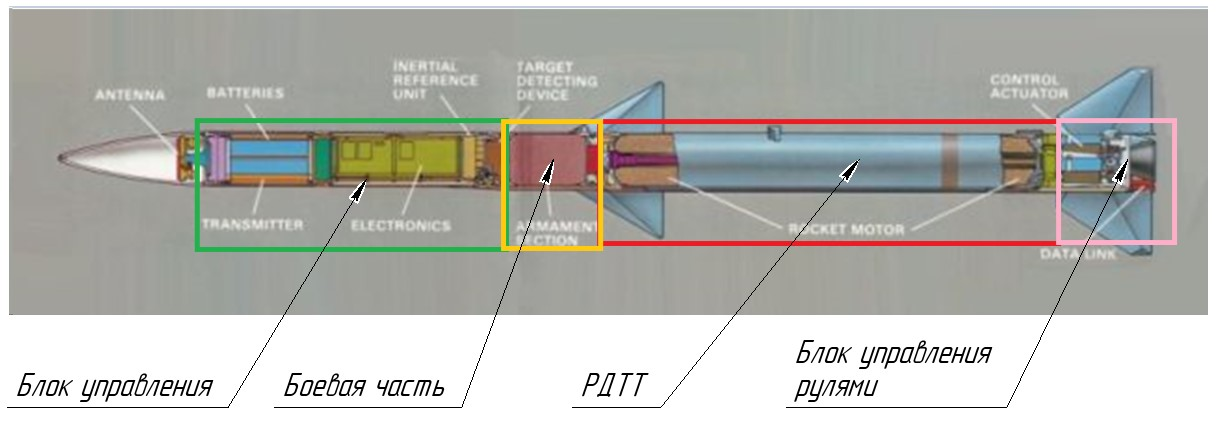
\includegraphics[width=0.65\textheight]{images/5.jpg}
\caption{Схема разбиения компоновки ракеты}
\label{AIM-120}
\end{figure}

\chapter{Массовый анализ}
\section{Расчёт масс отсеков из размеров ракеты}
Расчёт основан на имеющихся данных о массе ракеты, её боевой части из открытых источников. Масса РДТТ бралась из ДЗ по ПрРО предыдущего семестра. Масса остальных отсеков будет найдена
с помощью установленных зависимостей из [1].

Общая масса ракеты — 161.5 кг, масса БЧ — 22 кг. Масса РДТТ — 54.33 кг.

Первый шаг заключается в расчете общего объема ракеты на основе
указанных выше длины и калибра по следующей формуле

\[V = \frac{\pi D^2 L}{4} = \frac{\pi (0.58)^2 \cdot 12.81}{4} = \SI{3.38}{ft^3}\]

Для того что
бы получить оценочное значение массы, выбирается уравнение 4 из ана
лиза общей массы УРВВ:
\[W = 142.2\cdot(V)^{0.74},\]
\[W = 142.2 \cdot (3.38)^{0.74} = 350.18\text{ фунтов}(158.83\text{ кг})\] 

Данное оценочное значение может быть проверено с помощью уравне
ния 17, разработанного для ракет средней дальности:

\[ W = 177.5\cdot(V)^{0.73} \]

\[ W = 177.5\cdot(3.38)^{0.73} = 431.82 \text{ фунтов}(195.87\text{ кг}) \]

 Поскольку полученные значения отличаются, проводится сравнение со
ответствия для каждого из них. Выбирается уравнение 4, по причине более высокого значения R — квадрат. Таким образом, значение массы при
 начальной оценке равно 350.18 фунтов (158.83 кг). Следовательно, при из
вестных массе и объеме общая плотность изделия может быть рассчитана
 с помощью уравнений:30,


\[ \textit{DENS} = \frac{\textit{W}}{\textit{V}} \]

\[ \textit{DENS} = 103.6 \, \frac{\text{фунтов}}{\text{фут}^3} . \]

Затем вводятся уравнения, разработанные для масс отсеков с параметрами, которые были выведены и оценены. Во-первых, масса отсека ДУ
может быть оценена с помощью уравнения 77:

\[ \textit{PWt} = -284.9 + 633.6(D) - 0.105(W) + 0.949(\textit{DENS}); \]
\[ \textit{PWt} = -284.9 + 633.6(0.58) - 0.105(350.18) + 0.949(103.6) = 169.75 \text{ фунтов}\]


Данное значение проверяется уравнением 82:

\[ \textit{PWt} = 1548.0 - 43.7(L) - 1253.9(D) + 1.4(W) - 6.0(\textit{DENS}); \]
\[ \textit{PWt} = 1548.0 - 43.7(12.81) - 1253.9(0.58) + 1.4(350.18) - 6.0(103.6) = 129.593 \text{ фунтов} \]

............................................................................................................

Эти уравнения дали большое расхождение. Так как уравнение
77 имеет лучшее соответствие и меньшее значение MAE, для определения
массы отсека ДУ будет использоваться значение 350.18 фунтов (158.83 кг).
Теперь, зная массу отсека, можно определить его объем с помощью уравнения 22, разработанного для РВВ:

\[ \textit{PWt} = 2.7 + 112(\textit{PVOL}); \]
\[ \textit{PVOL} = 1.54 \, \text{фут}^3 \, (0.044 \, \text{м}^3). \]

Снова проверяем значение с помощью уравнения 39:

............................................................................................................

 Масса и размер отсека наведения и управления будут оценены анало
гичным образом. Сначала оценочное значение будет получено с помощью
 уравнения, разработанного при анализе по диапазонам дальности. Так же
 будет использоваться значение, полученное с помощью уравнения, обла
дающего лучшим соответствием и более низким значением MAE. Оценка
 массы отсека будет получена из уравнения 85:

\[ GCWt = 117.6(D) + 1.6(R) - 0.14(\textit{DENS}); \]

\[ GCWt = 117.6(0.58) + 1.6(R) - 0.14(\textit{DENS}); \]


Это значение также проверяем с помощью уравнения 90:

\[ GCWt = 38.9(L) + 910.9(D) - 77.3(V) + 0.3(W) - 7.4(\textit{DENS}); \]

\[ GCWt = 170 \, \text{фунтов} \, (77.111 \, \text{кг}). \]

В силу наличия расхождения, дополнительная оценка будет найдена с

помощью уравнения 66:

\[ \frac{W_{gc}}{W_t} = \exp(-0.89 - 0.06(V)); \]

\[ \frac{W_{gc}}{W_t} = 0.317; \]

\[ GCWt = 132 \, \text{фунта} \, (59.874 \, \text{кг}). \]
\end{document}